% !TEX program = pdfLaTeX
 
\documentclass[12pt, letterpaper]{article}

 
\usepackage{amssymb,amsmath}       % for more math
\usepackage{fancyvrb}              % for fancy verbatim mode
\usepackage{xcolor}                % to use colours
\usepackage[margin=2cm]{geometry}  % page layout
\usepackage{graphicx}
\usepackage{array}

\usepackage[pdftitle={COMP4109 Assignment},
            pdfsubject={Carleton University, 
                        COMP4109, Fall 2018},
            pdfauthor={M. Jason Hinek}]%
            {hyperref}

\usepackage{lastpage}              % to find the last page
\usepackage{fancyhdr}              % fancy headers

\pagestyle{fancy}
\lhead{\large \textbf{COMP4109 - Assignment 1}}
\rhead{\large {\textbf{Due \textcolor{red}{Friday, Oct 12, Noon}}}}
\lfoot{Applied Cryptography}
\cfoot{}
\rfoot{\thepage\ of \pageref{LastPage}}


% Some macros
\newcommand{\answer}[1]{{\small{\color{blue}#1}}}
\renewcommand{\answer}[1]{}

% I don't like paragraphs indented   
\setlength\parindent{0pt}
 
% --------------------------------------------------------------------------- %   
\begin{document}

{\Large
\begin{tabular}{rm{6cm}rm{6cm}}
Name :  & {Alexa de Grandmont} & Name : & {David Nelson}           \\
ID :    & NUMBA WON!   & ID :   & 100988794
\end{tabular}
}

\bigskip
\hrule
\bigskip


You can work in groups of two for the assignments. Each group will submit a single
typeset hardcopy of your solution to the SCS drop-boxes in HP 3115 by the deadline. Be sure to include the name and student id for
each person working on the assignment.  

\bigskip
\hrule
\bigskip

Some conventions used in the assignment:
\begin{itemize}\itemsep0cm
\item $\mathbb{Z}_N$ is the set of integers modulo $N$. It is the set $\{0,1,2,\dots,N-1\}$. 
\item $\mathbb{N}$ is the set of natural numbers $\{0,1,2,\dots\}$.
\item $X || Y$ is the concatenation of $X$ and $Y$.
\end{itemize}

\hrule

% ------------------------------------------- %
% ------------------------------------------- %
% ------------------------------------------- %
\section{DES2}
Consider a new block cipher, DES2, that consists only of two rounds of the Feistel structure (compared to 16 rounds for the noemal use of DES) of DES.  
DES2 has the same block and key size as DES. 
For this question, you should consider the DES round function $F$ 
as a black box that takes two inputs, a 32-bit data segment and
a 48-bit round key, and produces a 32-bit  output. Do not look inside the S-boxes for this problem. Do not look at the key scheduling algorithm for this problem.\\

Suppose you have a large number of plaintext-ciphertext pairs for DES2 under a single unknown key. 
Give an algorithm for recovering the 48-bit round key for round 1 and the 48-bit round key for round 2.
Your algorithm should require fewer operations than an exhaustive search for the entire 56-bit DES key. \\

Note: Problem taken from Cryptography Engineering by Ferguson, Schneier and Kohno.


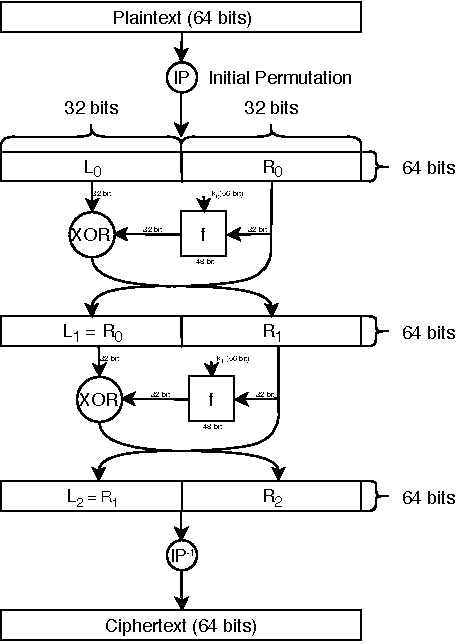
\includegraphics[width=6cm]{4109fig1.pdf}


less than $2^{56}$, but maybe do $2^{48}$ for round1, and $2^{48}$ round 2 these together is $2^{49}$

//We have plaintext/ciphertext pairs, i.e. we know many input sequences $L_0$ and $R_0$, and their corresponding outputs $L_2$ and $R_2$. We also know $L_1 = R_0$ and $L_2 = R_1$. 
$L_2 = R_1 = L_0 XOR f(R_0,K_0)$
$L_2 XOR L_0 = f(R_0,K_0)$
Since we know $L_2, L_0, and R_0,$, we can brute force $K_0$ by running f on $R_0$ and all possible key inputs to the function (these are of bitlength 48). We do this at most $2^48$ times. 

Similarly, we have that $R_2 = L_1 XOR f(R_1,K_1)$
$R_2 = R_0 XOR f(L_0 XOR f(R_0,K_0),K_1)$
$R_2 XOR R_0 = f(L_0 XOR f(R_0,K_0),K_1)$
Since we found $K_0$ earlier, we can compute $L_0 XOR f(R_0,K_0)$. Now the only unknown in the equation is $K_1$. As we did for $K_0$, we can also brute force $K_1$ by running f at most another $2^48$ times.

In total, the maximum number of operations we need to recover both 48-bit round keys is $2^48 + 2^48 = 2(2^48) = 2^49$, which is less than the $2^(56)$ operations required to brute force the 56-bit DES key.


% ------------------------------------------- %
% ------------------------------------------- %
% ------------------------------------------- %
\clearpage
\section{Pseudorandom Numbers}


One of the oldest pseudorandom number generators is the \emph{multiplicative congruence generator}.  For public $m \in \mathbb{N}$ and secrets $a,b_0 \in \mathbb{Z}_m$, the sequence of random 
numbers is generated using the recurrence  

\[ b_{i+1} = (a \times b_i) \bmod m,\]

for $i \geq 0$.
Show that the output of this PRNG is easily distinguished from a random sequence 
of numbers (modulo $m$).

\bigskip
Hint: Try to find some repeating mathematical relationship between several
elements in the output. The relationship should not explicitly have $a$ or $b_0$ in it. It can have the public parameter $m$ in it.

\bigskip
Note: If your answer relies on specific values of $a$ or $b_i$ or $m$, or if it relies on $m$ being small enough to observe a cycle (when the output repeats itself) then this is not what we are looking for.  

\bigskip
Solution: 

\[ b_{i-1} \times b_{i+1} \]
\[ = b_{i-1} \times (a \times b_{i}) \]
\[ = (a \times b_{i-1}) \times  b_{i} \]
\[ = b_{i} \times  b_{i} \]
\[ = (b_{i})^2 \]

//put some more (mod m) 's in there 

//mathematical relationship between every 3 consecutive "random" elements implies that this PRNG does not generate a random sequence of numbers 


% ------------------------------------------- %
% ------------------------------------------- %
% ------------------------------------------- %
\clearpage
\section{Hash Functions}

Let $f$, $g$ and $h$ be hash functions that each map binary strings of length $2n$ to binary strings of length $n$.  Suppose that  $h(x) = f( g(x) || g(x) )$, where $a||b$ means $a$ concatenated with $b$.  
Prove that if $f$ and $g$ are collision resistant then $h$ is also collision resistant. 

[Hint: review COMP1805 proof techniques.]\\
\\
if $f() \land g() \in CR$ , then $h() \in CR$ \\
by contrapositib
\\
$x \ne x'$ \\ 
$h(x)=h(x')$ \\
$h(x)=f(g(x)||g(x))$ \\
$h(x')=f(g(x')||g(x'))$ \\
$f(g(x)||g(x))=f(g(x')||g(x'))$ \\
$f^{-1}(g(x)||g(x))=f^{-1}(g(x')|| g(x'))$ \\
$g(x)||g(x)=g(x')||g(x')$ \\
$g(x)=g(x')$ \\
$g()$ is not collision resistant


% ------------------------------------------- %
% ------------------------------------------- %
% ------------------------------------------- %
\clearpage
\section{Bad Shuffles}
 
Consider the following card shuffling algorithm.  There are three cards in the deck and they are each represented by an element in $\{X,Y,Z\}$.  [\textcolor{blue}{Bonus marks if you use the deck $\{W,X,Y,Z\}$}] 

{\small
\begin{Verbatim}
   Algorithm Shuffle
   ---------------------------------------------------
   deck := [X,Y,Z]

   for i from 0 to 2 do
      j := RANDOM(i)
      swap values of deck[i] and deck[j]
   end for

   return deck
   ---------------------------------------------------
\end{Verbatim}
}

For each of the following definitions of \texttt{RANDOM(i)}, 
compute the probability distribution of all six valid hands, $[X,Y,Z]$, $[X,Z,Y]$, $[Z,X,Y]$, etc., at the end of the algorithm. Show your work. 

\begin{itemize}
\item[a)] \texttt{RANDOM(k)} returns an integer chosen uniformly at random from the set $\{0,1,2\}$.  Here, any of the three possibilities are equally returned.

\item[b)] \texttt{RANDOM(k)} returns an integer chosen uniformly at random from $k$ to $2$ (inclusive).  Here, values less than $k$ are not returned.

\item[c)] \texttt{RANDOM(k)} returns an integer chosen uniformly at random from the 
set $\{0,1,2\} \setminus \{k\}$. Here, the value of $k$ is never returned.
\end{itemize}
Your answer should give the probability of each possible hand.
Briefly comment about the results of the three algorithms. \\

Hint: Draw a tree starting with the un-shuffled deck $[X,Y,Z]$ where 
the different outputs of the \texttt{RANDOM} function yield a child (modified deck). The leaves are the tree are possible hands. The probability of a leaf node (specific hand) is the product of the probabilities of the nodes on the path from the root to that leaf.


\bigskip
Example: Suppose we use the functon \texttt{RANDOM(k) -> k}. The probability distribution is given by

{\small
\begin{align*}
\Pr\{ [X,Y,Z] \} = 1 \\
\Pr\{ [X,Z,Y] \} = 0 \\
\Pr\{ [Y,X,Z] \} = 0 \\
\Pr\{ [Y,Z,X] \} = 0 \\
\Pr\{ [Z,X,Y] \} = 0 \\
\Pr\{ [Z,Y,X] \} = 0
\end{align*}
}


Note: Drawing the probability trees in \LaTeX\, probably using TikZ, while looking amazing, will suck your time. I would recommend hand-drawing, scanning and then embedding the image. 

Solution: 

//Figure 1 (random A tree) here

{\small
\begin{align*}
\Pr\{ [X,Y,Z] \} = 4\left(\frac{1}{3} \right)^3 = \frac{4}{27} \\
\Pr\{ [X,Z,Y] \} = 5\left(\frac{1}{3} \right)^3 = \frac{5}{27} \\
\Pr\{ [Y,X,Z] \} = 5\left(\frac{1}{3} \right)^3 = \frac{5}{27} \\
\Pr\{ [Y,Z,X] \} = 5\left(\frac{1}{3} \right)^3 = \frac{5}{27} \\
\Pr\{ [Z,X,Y] \} = 4\left(\frac{1}{3} \right)^3 = \frac{4}{27} \\
\Pr\{ [Z,Y,X] \} = 4\left(\frac{1}{3} \right)^3 = \frac{4}{27} \\
\end{align*}
}

//Figure 2 (random B tree) here

{\small
\begin{align*}
\Pr\{ [X,Y,Z] \} = \left(\frac{1}{3} \right)\left(\frac{1}{2} \right)(1) = \frac{1}{6} \\
\Pr\{ [X,Y,Z] \} = \left(\frac{1}{3} \right)\left(\frac{1}{2} \right)(1) = \frac{1}{6} \\
\Pr\{ [X,Y,Z] \} = \left(\frac{1}{3} \right)\left(\frac{1}{2} \right)(1) = \frac{1}{6} \\
\Pr\{ [X,Y,Z] \} = \left(\frac{1}{3} \right)\left(\frac{1}{2} \right)(1) = \frac{1}{6} \\
\Pr\{ [X,Y,Z] \} = \left(\frac{1}{3} \right)\left(\frac{1}{2} \right)(1) = \frac{1}{6} \\
\Pr\{ [X,Y,Z] \} = \left(\frac{1}{3} \right)\left(\frac{1}{2} \right)(1) = \frac{1}{6} \\
\end{align*}
}

//Figure 3 (random C tree) here

{\small
\begin{align*}
\Pr\{ [X,Y,Z] \} = 0\left(\frac{1}{2} \right)^3 = 0 \\
\Pr\{ [X,Z,Y] \} = 3\left(\frac{1}{2} \right)^3 = \frac{3}{8} \\
\Pr\{ [Y,X,Z] \} = 3\left(\frac{1}{2} \right)^3 = \frac{3}{8} \\
\Pr\{ [Y,Z,X] \} = 0\left(\frac{1}{2} \right)^3 = 0 \\
\Pr\{ [Z,X,Y] \} = 0\left(\frac{1}{2} \right)^3 = 0\\
\Pr\{ [Z,Y,X] \} = 2\left(\frac{1}{2} \right)^3 = \frac{1}{4} \\
\end{align*}
}

//Comment about how we'd expect randomA to be more random than randomB

% ------------------------------------------- %
% ------------------------------------------- %
% ------------------------------------------- %
\clearpage
\section{Output Bias in RC4}
This problem involves a bias in the key-stream output of RC4.  
The key-scheduling algorithm and key-stream generator algorithm are given at the end of this assignment for reference. 

\begin{itemize}
\item[a)] Compute the second key-stream byte of the output when the input to the key-stream generator satisfies (S[1] != 2) and  (S[2] == 0). Show your work.

\item[b)] Estimate the probability that the second key-stream byte of RC4 is 0.  State any assumptions that you make.  (Your probability determination should be taken over all possible secret keys.)  What does your result show?
\hfill [Hint: In part (a), the second byte should be 0.]

\item[c)] Suppose a single 5-byte message $m$ is encrypted with many different RC4 secret keys and you are given all of the ciphertexts.  How can you use your result of part b) in this situation? What can you likely learn about the plaintext?
\end{itemize}
Solution a):
\begin{quote}

\begin{Verbatim}

i := 0; j := 0;
while NeedMoreBytes do
    i := 1
    j := a
    swap S[i] and S[j] : (S[1] is a, S[a] is 1)
    K := S[a+1] (S[a] is 1)
    return S[a+1]
end while

i=1;j=a;
while NeedMoreBytes do
    i := 2
    j := a + S[2] 
    swap S[2] and S[a] : (S[2] is a, S[a] = 0)
    K := S[a] (S[a] is 0)
    return S[a+1]
end while

After two iterations of NeedMoreBytes, S[1] != 2, S[2] is 0. The fact that i can never 
revisit an index it has already visited, is a weakness. 

NOTES: the first such result was shown by Mantin and Shamir who showed that the second
byte of RC4 PRGA is highly biased to be the byte 0. If the PRGA output was uniformly 
random, one would expect that any byte could be produced with probability 1/256. 
However, this result showed that the second byte is 0 with probability 1/128 (i.e. 
double the probability), and this is independent of the secret key.

\end{Verbatim}
\end{quote}
\clearpage
Solution b):

In our example, S has 256! possible permutations.\\
When $S_0$, the initial permutation follows the sequence of events outlined in our solution to part a, $S_0[2] = 0 $ and $S_0[1] != 2$, we can guarantee the second key-stream byte be 0 with a probability of 1 for $255!/256! = 1/256$ of all possible permutations. If $S_0[2] != 0 $, then we cannot guarantee which key-stream byte is the value $0$, but we do know that $S_0$ is uniformly distributed, so the second output value to be 0 has probability $1/256$ for $1-1/256 = 255/256$ of all possible permutations.

The probability determination taken over all possible secret keys relies on two events A and B. \\
Let $A$ be the event that the second key-stream byte is 0.\\
Let $B$ be the event that $S_0[2]=0$ is guaranteed.

\begin{align*}
& Pr(A) = Pr(A|B) * Pr(B) + Pr(A|\neg B) * Pr(\neg B)\\
& = 1 * 1/256 + (1-1/256) * 1/256\\
& = 1/256 + 255/256 * 1/256\\
& = 1/256 + 255/256^2\\
& = 256/256^2 + 255/256^2\\
& \approx 2(256)/256^2\\
& \approx 2/256
\end{align*}

This shows that there is a bias towards the second key-stream byte having a value of 0, and that the probability of this result is two-times the probability than an evenly distributed value. Although this bias shows twice the probability, if $n$ is large enough, then the relative probability is slight.\\
\\
Solution c):

We interpret many to be enough to apply the pigeon hole principal to force a collision.. 

\clearpage

\appendix
\subsection*{RC4}


{\small
\begin{Verbatim}
RC4 Key-schedule algorithm  (input: key)
---------------------------------------------------
for i from 0 to 255 do
    S[i] := i
end for

j := 0
for i from 0 to 255 do
    j := (j + S[i] + key[i % key.length]) % 256
    swap values of S[i] and S[j]
end for
---------------------------------------------------



RC4 Key-stream generator  (input: S[0],...,S[255])
---------------------------------------------------
i := 0
j := 0
while NeedMoreBytes do
   i := (i + 1) % 256
   j := (j + S[i]) % 256
   swap values of S[i] and S[j]
   K := S[(S[i] + S[j]) % 256]
   output K
end while
---------------------------------------------------
\end{Verbatim}
}


% --------------------------------------------------------------------------- %   
\end{document}
% --------------------------------------------------------------------------- %   